\section*{IO.I-1}
\subsection*{(i)}
In this problem, we will show that when $m = M/B + 1$, if we have the optimal replacement policy, then it performs only $O(n/B + \sqrt(n))$ I/Os.\\

Indeed, when $M > B$ (which is obvious) and $m > M$, the array can be separated into blocks as being shown in figure \ref{fig:row-major}. \\

\begin{figure}
  \centering
  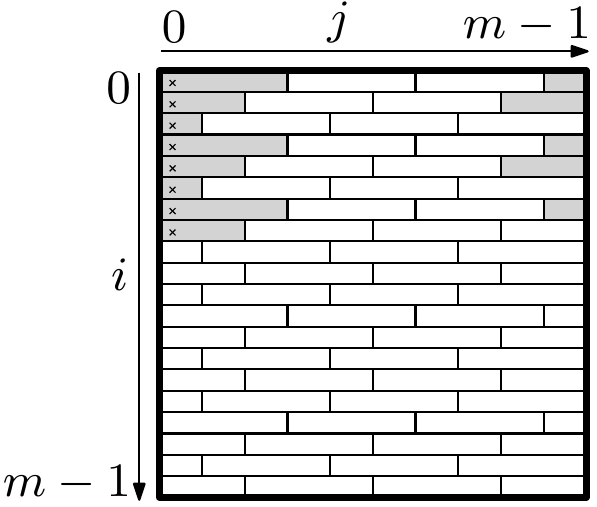
\includegraphics[width=0.5\textwidth]{row-major}
  \caption{Blocks loaded into an 2-dimensional array}
  \label{fig:row-major}
\end{figure}

Basically, we move in the column order, then each step in the first column requires an I/O. In each column, after filling the memory, there are several items left which total size is less than $B$. This is when we need the replacement policy. The optimal replacement method (sometimes called $MIN$) removes the block that has the longest time to be reused again in the future. In this particular setting, the $OPT$ will remove the block which the last item has the smallest index. E.g. the $3^{rd}$ selected block in figure \ref{fig:row-major}.\\

If $B$ does not divides $m$, then each column in the array has $(m - 1) / B$ blocks which the last item index is that column index, which are also the blocks that have the longest time to be reused in the future. Moreover, these blocks are indeed never used again in the same row. Therefore, the number of I/Os that $MIN$ performs is equal to the number of I/Os that the row order performs, plus an extra number of I/Os for the remaining column of size $s < B$ (because $B$ does not divides $m$).\\

We have $m$ rows, and $m/B + 1$ I/Os for each row. Thus the number of I/Os is:

 $$(\frac{m}{B} + 1)m = O(\frac{n}{B} + \sqrt{n})$$

If $B$ divides $m$, then we do not have the distribution as being shown in figure \ref{fig:row-major}. Instead, all loaded blocks in a columns have the same ending index. Then the optimal replacement here is the Most Recently Used, that is, the policy evicts the latest used block. The array is now divided into $m / B$ columns of size $B$. Each such column requires $m$ I/Os for the first ``real'' column, and 1 I/O for each of the remaining columns. In general, the number of I/Os is:

$$\frac{m}{B}(m + B - 1) = \frac{m^2}{B} + \frac{m(B - 1)}{B} = O(\frac{n}{B} + \sqrt{n})$$

\subsection*{(ii)}
In case $m > 2M/B$ and $m$ is significantly larger than $M$, then each column of the array can store at least 2 memory-size regions, plus several individual items. \\

If we traverse the array in column-major order and the OS uses the optimal replacement strategy, then at the end of each column, all elements in the first $M-size$ part has been removed to get the space for the latest elements in the column. Therefore, whatever replacement method we use (even the optimal one), we cannot reuse any block when we move to the next column. Therefore, we need to load a new block everytime we want to fetch a new item. Thus, the I/O complexity is $\Omega(n)$.\\

If the OS uses the Most Recently Used replacement policy, then we can keep $m/2$ items for the first column, but we have to load-and-clear every item in the remaining $m/2$ items. Therefore, the I/O complexity is still a factor of $m^2$, which is $\Omega(n)$.
